%%%%%%%%%%%%%%%%%%%%%%%%%%%%%%%%%%%%%%%%%%%%%%%%%%%%%%%%%%%%%%%%%%%%%%%%%%%%%%%%%%%%%%%%%%%%%%%%%%%%%%%%%%%%%%%%%%%%%%%%%%%%%%%%%%%%%%%%%%%%%%%%%%%%%%%%%%%%%%%%%%%
% Written By Michael Brodskiy
% Class: Fundamentals of Networks
% Professor: E. Bernal Mor
%%%%%%%%%%%%%%%%%%%%%%%%%%%%%%%%%%%%%%%%%%%%%%%%%%%%%%%%%%%%%%%%%%%%%%%%%%%%%%%%%%%%%%%%%%%%%%%%%%%%%%%%%%%%%%%%%%%%%%%%%%%%%%%%%%%%%%%%%%%%%%%%%%%%%%%%%%%%%%%%%%%

\documentclass[12pt]{article} 
\usepackage{alphalph}
\usepackage[utf8]{inputenc}
\usepackage[russian,english]{babel}
\usepackage{titling}
\usepackage{amsmath}
\usepackage{graphicx}
\usepackage{enumitem}
\usepackage{amssymb}
\usepackage[super]{nth}
\usepackage{everysel}
\usepackage{ragged2e}
\usepackage{geometry}
\usepackage{multicol}
\usepackage{fancyhdr}
\usepackage{cancel}
\usepackage{siunitx}
\usepackage{physics}
\usepackage{tikz}
\usepackage{mathdots}
\usepackage{yhmath}
\usepackage{cancel}
\usepackage{color}
\usepackage{array}
\usepackage{multirow}
\usepackage{gensymb}
\usepackage{tabularx}
\usepackage{extarrows}
\usepackage{booktabs}
\usepackage{lastpage}
\usepackage{float}
\usetikzlibrary{fadings}
\usetikzlibrary{patterns}
\usetikzlibrary{shadows.blur}
\usetikzlibrary{shapes}

\geometry{top=1.0in,bottom=1.0in,left=1.0in,right=1.0in}
\newcommand{\subtitle}[1]{%
  \posttitle{%
    \par\end{center}
    \begin{center}\large#1\end{center}
    \vskip0.5em}%

}
\usepackage{hyperref}
\hypersetup{
colorlinks=true,
linkcolor=blue,
filecolor=magenta,      
urlcolor=blue,
citecolor=blue,
}


\title{Computing Homework 2}
\date{October 30, 2023}
\author{Michael Brodskiy\\ \small Professor: E. Bernal Mor}

\begin{document}

\maketitle

\begin{figure}[H]
  \centering
  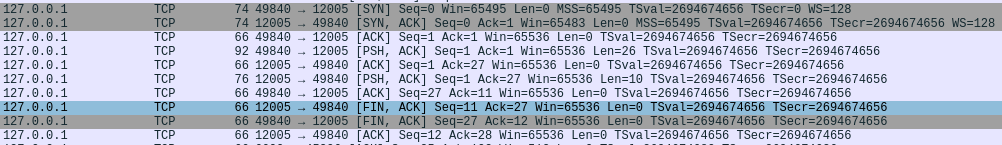
\includegraphics[width=.9\textwidth]{Figures/Capture.png}
  \caption{A Screenshot of Packet Capture}
  \label{fig:1}
\end{figure}

\begin{enumerate}

  \item From the above capture, we may see that there are two packets exchanged to establish a connection. The first, which we can see originates from the client ($49840\to12005$) initiates the connection. This is indicated by the $\left[ \text{\textsc{SYN}} \right]$ flag, or synchronize, being set to 1, which essentially asks the server to connect. The server replies ($12005\to49840$) with a packet of $\left[ \text{\textsc{SYN, ACK}} \right]$, both set to 1, which signifies that the connection may be established, and the server acknowledges the receipt of the first packet.

  \item We can see that the port number of the client is $49840$. We know this because the two ports involved are $12005$ and $49840$, and we know that the client can not be $12005$, since we set the server port number to that value. Thus, the client must be $49840$.

  \item We can identify the segments that carry data by the Push field, or rather $\left[ \text{\textsc{PSH}} \right]$ flag, being set to 1. We can thus see, that there are two such packets, one sent to the server (carrying the numerical combination), and one sent to the client (carrying the \textsc{RESULT:X} data). We can identify the amount of ``bytes on wire'' by looking at the length descriptor of each of those packets. Thus, we can see that the data packet from the client to the server is 92 bytes in length, and the data packet from the server to the client is 76 bytes.

  \item The message sent from the client to the server is the one of length 92. The actual ASCII encoding is:


    \begin{center}
      \begin{array}{l l l}
        0000&\text{00 00 00 00 00 00 00 00 00 00 00 00 08 00 45 00}&\text{..............E.}\\
        0010&\text{00 4e a3 0d 40 00 40 06 99 9a 7f 00 00 01 7f 00}&\text{.N..@.@.........}\\
      0020&\text{00 01 c2 b0 2e e5 76 7d 11 ba d0 8d 5c a9 80 18}&\text{......v\}....\\...}\\
      0030&\text{02 00 fe 42 00 00 01 01 08 0a a0 9d 78 e0 a0 9d}&\text{...B........x...}\\
      0040&\text{78 e0 31 32 2d 32 33 2d 35 36 2d 35 2d 39 35 2d}&\text{x.12-23-56-5-95-}\\
      0050&\text{33 2d 35 35 2d 32 34 2d 39 2d 33 34}&\text{3-55-24-9-34}\\
      \end{array}
    \end{center}

    We can see the actual string of numerical values following the header of this packet in the last two lines of the ASCII encoding.

\end{enumerate}

\end{document}

